%\documentclass[a4paper,11pt,fleqn]{article}
\documentclass[10pt,fleqn,twocolumn]{IEEEtran}
\usepackage{amsfonts}
\usepackage{amsthm}
\usepackage{graphicx}

\usepackage{/usr/share/texmf/tex/latex/cite/cite}

\setlength{\parindent}{1em}
\setlength{\oddsidemargin}{0in}
\setlength{\textwidth}{6.5in} % sets 1in left and right margins
\setlength{\topmargin}{0.5in} % change to 0.2in for regular latex
%\setlength{\headheight}{0in}
%\setlength{\footheight}{0.5in}
\setlength{\footskip}{0.5in}
\setlength{\textheight}{9.0in} %sets 1in top and bottom margins


\newtheorem{Prop}{Proposition}
\newtheorem{lemma}{Lemma}

\newcommand{\br}{{\mathbf r}}
\newcommand{\bA}{{\mathbf A}}
\newcommand{\ba}{{\bf a}}
\newcommand{\bb}{{\bf b}}
\newcommand{\bc}{{\bf c}}
\newcommand{\bC}{{\bf C}}
\newcommand{\bd}{{\bf d}}
\newcommand{\be}{{\bf e}}
\newcommand{\bs}{{\bf s}}
\newcommand{\bm}{{\bf m}}
\newcommand{\bn}{{\bf n}}
\newcommand{\bu}{{\bf u}}
\newcommand{\bv}{{\bf v}}
\newcommand{\bw}{{\bf w}}
\newcommand{\bx}{{\bf x}}
\newcommand{\bz}{{\bf z}}
\newcommand{\bbf}{{\bf f}}
\newcommand{\bL}{{\bf L}}
\newcommand{\bM}{{\bf M}}
\newcommand{\bN}{{\bf N}}
\newcommand{\bS}{{\bf S}}
\newcommand{\bT}{{\bf T}}
\newcommand{\bD}{{\bf D}}
\newcommand{\bX}{{\bf X}}
\newcommand{\bP}{{\bf P}}
\newcommand{\bI}{{\bf I}}
\newcommand{\bR}{{\bf R}}
\newcommand{\bU}{{\bf U}}
\newcommand{\bV}{{\bf V}}
\newcommand{\bW}{{\bf W}}
\newcommand{\bJ}{{\bf J}}
\newcommand{\bB}{{\bf B}}
\newcommand{\bzero}{{\bf 0}}
\newcommand{\bgamma}{{\mbox {\boldmath $\gamma$}}}
\newcommand{\btheta}{{\mbox {\boldmath $\theta$}}}
\newcommand{\bLambda}{{\mbox {\boldmath $\Lambda$}}}
\newcommand{\bPsi}{{\mbox {\boldmath $\Psi$}}}
\newcommand{\bPhi}{{\mbox {\boldmath $\Phi$}}}
\newcommand{\bcS}{{\mbox {\boldmath ${\cal S}$}}}
\newcommand{\bcH}{{\mbox {\boldmath ${\cal H}$}}}
\newcommand{\bcI}{{\mbox {\boldmath ${\cal I}$}}}
\newcommand{\bcR}{{\mbox {\boldmath ${\cal R}$}}}
\newcommand{\bcB}{{\mbox {\boldmath ${\cal B}$}}}

\title{Semi-Blind Decorrelating Multiuser Detection for Synchronous CDMA}
\date{}
\author{S. Wang, J. Caffery, Jr. and H. Shen\\ Department of
ECECS \\ University of Cincinnati \\ Cincinnati, OH~~45221-0030}
%\\ \{{\tt swang,jcaffery, shenhg\}@ececs.uc.edu}}

\begin{document}
\maketitle

\begin{abstract}
Multiuser detection is a key technology for combating multiple
access interference (MAI) in CDMA systems. In this paper, we
propose three effective one-shot multiuser semi-blind
decorrelating detectors based on least squares (LS), total least
squares (TLS) and mixed LS/TLS (MLS) formulations. All of the
proposed algorithms are based on the classic decorrelating
detector and a new semi-blind signature matrix. Different
assumptions regarding the noise in the proposed semi-blind
signature matrix lead to different detection algorithms. We also
find that the classic decorrelating detector can be regarded as a
special case of the proposed LS decorrelating detector. The
proposed detection algorithms are simple and direct, where only
the timing, signature and amplitude of the desired user are
required. In addition, no search or convergence procedure is
required. Finally, theoretical analysis and computer simulations
are presented to illustrate the performance of the proposed
algorithms.
\end{abstract}

\section{Introduction}

Multiuser detection is a strategy for minimizing the effect of MAI
and mitigating the near-far problem, especially in CDMA systems.
MAI is the dominant impairment for CDMA systems and exists even in
perfect power-controlled CDMA systems. Most early work on
multiuser detection assumed that the receiver had some knowledge
of the users' timing, received amplitude and/or signature waveform
which was exploited to combat MAI.  For example, the classic
decorrelating detector can achieve the optimum near-far resistance
and completely eliminate MAI at the expense of background noise
enhancement. Though the decorrelating detector does not require
knowledge of all users' received amplitudes, it does require
information about their signature waveforms. However, in many
practical cases, especially in a dynamic environment, it is very
difficult for a mobile user to obtain accurate information of
other active users.
%On the other hand, the frequent use of training sequences
%is certainly a waste of channel bandwidth.
Most of the multiuser detection schemes assume knowledge of the
spreading codes and/or channel parameters of all the users that
contribute to the received signal. Blind detectors, on the other
hand, operate without knowledge of the channel or information of
other users. Usually, many practical systems lie in between these
two extremes. The first form of detectors are too optimistic as we
cannot expect to know the signature waveforms or received
amplitudes of all the users, especially in the downlink of a CDMA
system, while the latter under-utilizes the knowledge of the
system.

Recent research has been devoted to blind multiuser receivers and
subspace-based signature waveform estimation schemes to achieve better
performance and higher capacity~\cite{Honi95,Poor97,Wang98,Torl97,Liu96}.
The minimum output energy (MOE) method and subspace methods were
presented for multiuser blind detection with the knowledge of only
the desired users' spreading code and possible timing.
%It is shown
%in~\cite{Honi95} that the blind MOE receiver is equivalent to the
%linear minimum mean square error (MMSE) detector, which is
%near-far resistant and has much less complexity compared the
%optimal multiuser detection.
In the subspace-based blind detection approach~\cite{Wang98}, the
linear detectors offer lower computational complexity and better
performance than the blind MOE detector. However, the signal
subspace components need to be computed before detection.

In this work, we consider a synchronous DS-CDMA system and develop
a least squares multiuser semi-blind decorrelating detector
(LS-DD), a total least squares multiuser semi-blind decorrelating
detector (TLS-DD), and a mixed LS/TLS multiuser semi-blind
decorrelating detector (MLS-DD). The detectors are semi-blind
since they require the signature waveform and received amplitude
of the desired user (timing is inherently assumed). A new
semi-blind signature matrix is proposed on which the decorrelating
operation is based. All algorithms are one-shot algorithms. No
knowledge of the other users' information is required and no
search or convergence procedure is employed. Theoretical analysis
and computer simulations are also presented to demonstrate the
performance of the proposed multiuser detectors. It is expected
that these proposed algorithms can bridge the performance gap
between the blind and the conventional multiuser detectors.

\section{Data Model and Problem Description}

The basic CDMA $K$-user channel model, consisting of the sum of
antipodally modulated synchronous signature waveforms embedded in
additive white Gaussian noise (AWGN), is considered here. The
received base-band signal during one symbol interval in such a
channel can be modeled as
\begin{equation}
\matrix{r(t)=\sum\limits_{k=1}^{K}A_k b_k s_k (t)+ n(t)}
\end{equation}
where $K$ is the number of users, $A_k$ and $b_k$ denote
the received amplitude and $n$th data bit for the $k$th user,
respectively, $n(t)$ represents the Gaussian channel noise, and $T$ is
the symbol interval. It is assumed that $b_k\in\{-1,\ +1\}$ is a
collection of independent, equiprobable random variables and $s_k(t)$
denotes the normalized signal waveform of the $k$th user during the
interval $t\in [(n-1)T,\ nT]$, i.e., $\|s_k(t)\|=1$.

The received signal, $r(t)$, is passed through a chip-matched filter
followed by a chip-rate sampler.  As a result, $r(t)$, $t\in
[(n-1)T,\ nT]$, is converted into a $L\times 1$ column vector,
$\br$, containing the samples of the chip-matched filter outputs within
the symbol interval $[(n-1)T,\ nT]$ as
%\footnote{Without loss of
%generality, the subscript index $n$ is dropped. Hence, it is
%assumed $\br=\br_n$ and $\bb=\bb_n$ .}
\begin{equation}
\br = \bS \bA \bb + \bn
\label{r}
\end{equation}
where $\bA=\mbox{diag}\{A_1\ A_2\ \ldots\ A_K\}$ is the diagonal
received amplitude matrix, $\bS = [\bs_1\ \bs_2\ \ldots\
\bs_K]$ is the $L \times K$ signature matrix with the $k$th column,
$\bs_k$, being the signature vector of the $k$th user, $\bb = [b_1\
b_2\ \ldots\ b_K]^T = [b_1\ \tilde{\bb}^T]^T$ is the vector containing data
sent by all the $K$ users at time $t=n$, and $\bn$ is an
$L$-dimensional Gaussian vector with independent $\sigma_n^2$-variance
components. We maintain the restriction that $L \geq K$.

Most linear multiuser detectors for demodulating the $k$th user's data
bit in (\ref{r}) is in the form of a correlator followed by a hard limiter,
which can be expressed as
\begin{equation}
\hat{b}_k = \mbox{sgn}\{\bw_k^T\br\},
\label{linear}
\end{equation}
where $\bw_k \in \mathbb{R}^{L\times 1}$ is the linear representation of
multiuser detector for user $k$.
%Linear multiuser detectors can be implemented in a decentralized
%fashion where only the user or users of interest need be
%demodulated.

\section{Decorrelating Detector}

%The large gaps in performance and complexity between the
%conventional single-user matched filter and optimum multiuser
%detector encourage the search for other multiuser detectors that
%exhibit good performance/complexity tradeoffs.
The decorrelating detector, one of the earliest suggestions to eliminate
multiuser interference with a linear receiver, was proposed by
Shnidman~\cite{Shni67}.
%The derivation of the asymptotic
%efficiency of the decorrelating detector for synchronous channels
%Tand the proof of its optimum near-far resistant property are due
%to Verd\'{u}~\cite{Verd86} in the case of nonsingular covariance
%matrices.
The forerunner of the decorrelating detector in the single-user
intersymbol interference (ISI) channel is the {\em zero-forcing equalizer}.
Further, the counterpart of decovariance in an antenna array subject to
undesired sources is called {\em null steering}.   Prior to developing the
semi-blind decorrelating detector, we first discuss decorrelating detection.

According to (\ref{r}), the classic decorrelating detector performs
the following operation:
\begin{equation}
\begin{array}{rcl}
\hat\bb&=&\mbox{sgn}\{\bW_{\rm DD}^{T}\br\}\\
 &=&\mbox{sgn}\{\bS^+\br\}
\end{array}
\end{equation}
where $\bW_{\rm DD}$ is the linear filter representation of the
decorrelating detector bank and $\bM^+$ denotes the
Moore-Penrose generalized inverse of the matrix $\bM$.

The decorrelating detector is one of the simplest multiuser
detectors and is designed to completely eliminate MAI caused by
the other users, but suffers from noise enhancement. When the
received amplitudes are completely unknown, the decorrelating
detector is a sensible choice.
%There are some desirable features of this
%multiuser detector.
Desirable properties of the detector include not requiring knowledge of
the received amplitudes, but it requires $\bS^+$. It can readily be
decentralized in the sense that the demodulation of each user can be
implemented separately.

\section{One-Shot Semi-blind Decorrelating Detection Schemes }

In this section, we develop three one-shot multiuser
semi-blind decorrelating detectors that are expected to bridge the
performance gap between the conventional and blind detectors.

\subsection{\em New Data Model with Semi-Blind Signature Matrix}

Without loss of the generality, we consider only the bit, $b_1$, sent by
the first user at time $t=n$. We first define a new $L\times M$
semi-blind signature matrix $\bcS$ for user $1$ which is constructed
as
%\footnote{Without loss of the generality, we use both $\bcS$ and $\bcS_1$ to
%represented the semi-blind signature matrix for user 1.}
\begin{equation}
\begin{array}{rcl}
\bcS&=&[\matrix{A_1\bs_1&\br_{1}&\br_{2}&\ldots&\br_{M-1}}]\\
 &=&\bS\bA\left[\matrix{\be_1&\bb_1&\bb_2&\ldots&\bb_{M-1}}\right]+ \bN\\
 &=&\bS\bA\left[\matrix{\be_1 & \bD }\right]+ \bN\\
 &=&\bS\bA\bB + \bN
\end{array} \label{S}
\end{equation}
where $\br_m$, $m=1,\ldots,M-1$, are $M-1$ previously received and
linearly independent blind vectors that are used to compose
$\bcS$, $\be_1$ is a $K\times 1$ identity vector with a $1$ on the
first row and $0$'s elsewhere, and the $K\times 1$ vectors $\bb_m$
are the corresponding data vectors which denote the unknown
information sent by all $K$ users in the previously received
vector $\br_m$ . The matrix $\bS$ is the original signature matrix
with the desired user's signature vector in the first column, $\bD
= [\bar{\bd}\ \tilde{\bD}^T]^T$ where the $(K-1)\times 1 $ vector
$\bar{\bd}$ is the data vector consisting of the known bits sent
by the desired user in previous signaling intervals.   Further,
note that $\mbox{rank} \{\tilde{\bD}\}=K-1$, $\bN=[\mathbf{0}\
\tilde{\bN}]$,
\begin{equation}
 \bB=\left[\matrix{1& \bar{\bd}^{T} \cr \mathbf{0}& \tilde{\bD} }\right]
\end{equation}
and $\mbox{rank}\{\bB\}=K$. %$L\geq M\geq K$.

From (\ref{r}) and (\ref{S}), the relationship between the received signal
vector, $\br$, and the new semi-blind signature matrix, $\bcS$, is
\begin{equation}
\br=\bcS\bd + \bz
\label{rn}
\end{equation}
where $\bd$ denotes a new $K \times 1$ detection vector defined as
\begin{equation}
\bd = \bB^{+}\bb = \left[\matrix{1&\bar{\bd}^T\cr\mathbf{0}&\tilde{\bD}}
\right]^{+}\left[\matrix{b_1\cr\tilde{\bb}}\right]
\label{DetectorVector}
\end{equation}
and $\bz$ is the new noise vector defined as
\begin{equation}
\bz = \bn-\bN\bB^{+}\bb \enspace.
\label{new_noise}
\end{equation}

%Now, the following theorem can be easily proven.
\begin{lemma}
The bit sent by the first user, $b_1$, during the time interval
$t\in[(n-1)T,\ nT]$ can be estimated as
\begin{equation}
b_1 =  \bc^T\bd
\end{equation}
where $\bc=[\matrix{1&\bar{\bd}^T}]^T$ and $\bd=\left[\matrix{d_1&\tilde{\bd}}
\right]^T$.
\label{bn_estimation}
\end{lemma}

With the definition of the new semi-blind signature matrix, $\bcS$, in
(\ref{S}), the new multiuser detection model in (\ref{rn}) remains in the
same form as (\ref{r}).  The difference is that the original signature
matrix, $\bS$, is replaced by the semi-blind signature matrix, $\bcS$,
the data vector $\bb$ is replaced by the detection vector
$\bd$ in (\ref{DetectorVector}), and the original AWGN vector $\bn$ is
replace by the new noise vector $\bz$ in (\ref{new_noise}).
Fortunately, with Lemma~\ref{bn_estimation}, it is possible to calculate
the desired bit $b_1$ with the detection vector $\bd$ and the previously
detected bit vector $\bc$.  The main question is how to estimate the
detection vector $\bd$ as efficiently as possible.  The following sections
propose three approaches that depend on assumptions regarding $\bN$
in the semi-blind signature matrix $\bcS$.

\subsection{\em LS Semi-Blind Decorrelating Detector}

We first assume that the received measurements in $\bcS$ are assumed to
be free of error.  Hence, all errors are confined to the received
vector $\br$ due to $\bz$ in (\ref{rn}) in the $n$th bit interval.  The
following LS estimator is proposed along the lines of the classic
decorrelating detector.

\begin{lemma}~\cite{Golu96} Suppose $\bU^T\bcS\bV=\mathbf{\Sigma}$ is the SVD of $\bcS\in\mathbb{R}^{L\times
 K}$ with $r=rank(\bcS)$.  If $\bU=[\bu_1\ \bu_2\ \ldots\ \bu_L]$,
 $\bV=[\bv_1\ \bv_2\ \ldots\ \bv_K]$, $\mathbf{\Sigma}={\rm diag}\{[\sigma_1\ \ldots\ \sigma_r\ 0\ \ldots\ 0]\}$ and $\br\in \mathbb{R}^{L\times 1}$, then
 \begin{equation}
 \matrix{\bd_{\rm LS} = \sum_{i=1}^{r} \frac{\bu_i^T\br}{\sigma_i} \bv_i =
 \bcS^+\br}
 \label{LS}
 \end{equation}
minimizes $\|\bcS\bd-\br\|_2$ and has the smallest 2-norm of all minimizers.
Moreover, the minimum squared error achieved is
\begin{equation}
\varepsilon_{\rm LS}^2=\min\limits_{\bx\in\mathbb{R}}\|\bcS\bx-\br\|_2^2=\sum\limits_{i=r+1}^{L} \left(\bu_i^T\br\right)^2 \enspace .
\end{equation}
\label{VectorLS}
\end{lemma}

%So, the least squares estimation of $\bd$ is
%\begin{equation}
%\begin{array}{rcl}
%\bd_{LS} &=& \bcS^+\br.
%\end{array} \label{LS}
%\end{equation}

The linear filter $\bw_{\rm LS}$ in the LS semi-blind decorrelating detector
for user 1 is then
\begin{equation}
\bw_{\rm LS} = \left(\bc^T\bcS^+\right)^T
\label{w_LS}
\end{equation}
so that the bit sent by the first user, $b_1$, in the $n$th signaling
interval is detected with
\begin{equation}
\begin{array}{rcl}
\hat{b}^{\rm LS}_{1}&=&\mbox{sgn}\{\bw_{\rm LS}^{T}\br\}\\
 &=&\mbox{sgn}\left\{b_1+\bc^T\bcS^+\tilde{\bn}\right\} \enspace .
\end{array} \label{b_LS}
\end{equation}

\subsection{\em TLS Semi-Blind Decorrelating Detector}

The previous LS estimate of the detection vector $\bd$ from (\ref{rn}),
(\ref{DetectorVector}) and (\ref{LS}) is the solution to
\begin{equation}
\begin{array}{rcl}
\hat{\bd}=\matrix{\min\limits_{\bx}\left\|\br-\bcS\bx\right\|_2}&\mbox{subject
to}&\br\subseteq \mathbb{R}(\bcS)
\end{array}
\label{LSProb}
\end{equation}
where the semi-blind signature matrix $\bcS$ is assumed to be error-free.
However, this assumption is not entirely accurate according to the
definition of $\bcS$ in (\ref{S}) since there is a noise term, $\bN$.

Furthermore, $\br$ can also be expressed as
\begin{equation}
\begin{array}{rcl}
\br&=&(\bcS-\bN)\bB^{+}\bb + \bn\\
 &=&\hat{\bcS}\bd + \bn
\end{array}
\end{equation}
where  $\hat{\bcS}=\bcS-\bN=\bS\bA\bB$.  The minimization problem of
(\ref{LSProb}) can then be transformed into the following TLS problem:
\begin{equation}
\begin{array}{rcl}
\left[\hat{\bcS},\ \bx\right]&=&\matrix{\min\limits_{\bar{\bcS},\
\bx}\left\|\left[ \matrix{\bcS&\br} \right] - \left[ \matrix{\bar{\bcS}&
\bar{\bcS}\bx}\right]\right\|_2}
\end{array},
\label{TLSProb}
\end{equation}
subject to $\br\subseteq\mathbb{R}(\bar{\bcS})$.

\begin{lemma}\cite{Huff91} Let $\bcS=\bU^{'}\mathbf{\Sigma}^{'}\bV^{'T}$ and
$[\bcS\ \br]=\bU\mathbf{\Sigma}\bV^T$ be the SVD of $\bcS$ and
$[\bcS\ \br]$, respectively. If $\sigma_K^{'}
> \sigma_{K+1}$, then
\begin{equation}
\bd_{\rm TLS} = \left(\bcS^T\bcS-\sigma_{K+1}^2\bI\right)^{-1}\bcS^T\br
\end{equation}
and
\begin{equation}
\begin{array}{rcl}
\varepsilon_{\rm TLS}^{2}&=&\min\limits_{\bx\in \mathbb{R}^{K\times
1}}\|\bcS\bx-\br\|_2^2 \\
 &=& \sigma_{K+1}^2\left[1+\sum_{i+1}^{K}\frac{\left(\bu_i^{'T}\br\right)^2}
{\sigma_i^{'2}-\sigma_{K+1}^2}\right]
\end{array}
\end{equation}
where $\bU=[\bu_1\ \bu_2\ \ldots\ \bu_L]$, $\bV=[\bv_1\
\bv_2\ \ldots\ \bv_{K+1}]$, $\mathbf{\Sigma}={\rm diag}\{[\sigma_1\
\sigma_2 \ldots\ \sigma_{K+\min\limits\{L-K,\ 1\}}]\}$ and
$\bU^{'}=[\bu_1^{'}\ \bu_2^{'}\ \ldots\ \bu_L^{'}]$,
 $\bV^{'}=[\bv_1^{'}\ \bv_2^{'}\ \ldots\ \bv_{K}^{'}]$,
 $\mathbf{\Sigma}^{'}={\rm diag}\{[\sigma_1^{'}\ \sigma_2^{'}\ \ldots\ \sigma_K^{'}]\}$.
\end{lemma}

%So, the total least squares estimation of $\bd$ is
%\begin{equation}
%\begin{array}{rcl}
%\bd_{TLS}&=&(\bcS^T\bcS-\sigma_{K+1}^2\bI)^{-1}\bcS^T\br
%\end{array}
%\end{equation}

The linear filter representation of the TLS semi-blind decorrelating
detector is
\begin{equation}
\bw_{\rm TLS} = \bcS(\bcS^T\bcS-\sigma_{K+1}^2\bI)^{-1}\bc
\end{equation}
and the bit sent by the first user, $b_1$, in the $n$th signaling interval
can be detected with
\begin{equation}
\begin{array}{rcl}
\hat{b}^{\rm TLS}_{1}&=&\mbox{sgn}\{\bw_{\rm TLS}^T\br\}\\
 &=&\mbox{sgn}\left\{ \bc^T\left(\bcS^T\bcS-\sigma_{K+1}^2\bI\right)^{-1}
 \bcS^T\br\right\} \enspace .
% &=&\mbox{sgn}\{b_n^1+[\matrix{A_1^{-1}&\bar{\bd}^T}]\bcS^+\tilde{\bn}\}
\end{array}
\label{b_TLS}
\end{equation}

\subsection{\em Mixed LS/TLS Semi-Blind Decorrelating Detector}

In the LS problem of (\ref{LSProb}), it assumed the
semi-blind signature matrix $\bcS$ is error-free. Again, this
assumption is not completely accurate. In the TLS problem of (\ref{TLSProb}),
it assumed that in each column of the semi-blind signature matrix, $\bcS$,
some noise or error exists.  This assumption also is not complete.
Though there exists a noise or error matrix $\bN$ in
$\bcS$ from (\ref{S}), its first column is exactly known to be noise-free
or error-free.  Hence, to maximize the estimation accuracy of the detection
vector $\bd$, it is natural to require that the corresponding columns
of $\bcS$ be unperturbed since they are known exactly. The problem  of
estimating the detection vector $\bd$ can then be transformed into the
following MLS problem by considering (\ref{LSProb}) and (\ref{TLSProb}):
\begin{equation}
\begin{array}{rcl}
\matrix{\min\limits_{\bar{\bcS},\
\bx}\left\|\left[\matrix{\tilde{\bcS}&\br}\right]-\left[\matrix{\bar{\bcS}&[A_1\bs_1\
 \bar{\bcS}]\bx}\right]\right\|_{2} }
\end{array}\label{MLSProb}
\end{equation}
subject to $\br\subseteq\mathbb{R}([A_1\bs_1\ \bar{\bcS}])$.  The following
lemma outlines the MLS solution.

\begin{lemma}~\cite{Huff91} Consider the MLS problem in (\ref{MLSProb})
and perform the Householder transformation $Q$ on the matrix
$[\matrix{\bcS&\br}]$ so that
\begin{equation}
\begin{array}{rcl}
Q^H[\matrix{A_1\bs_1&\bar{\bcS}&\br}]&=&\left[\matrix{R_{11}&\bR_{12}&R_{1r}\cr
\mathbf{0}&\bR_{22}&\bR_{2r}}\right]
\end{array}
\end{equation}
where $R_{11}\neq 0$, $\bR_{12}$ is a $1\times (M-1)$
vector, $\bR_{22}$ is a $(L-1)\times (M-1)$ matrix and $\bR_{2r}$
is a $(L-1)\times 1$ vector.

Denote $\sigma'$ as the smallest singular value of $\bR_{22}$ and
$\sigma$ as the smallest singular value of $[\matrix{\bR_{22}&\bR_{2r}}]$.
If $\sigma'>\sigma$, then the MLS solution uniquely exists and is given by
\begin{equation}
\begin{array}{rcl}
\bd_{\rm MLS}&=&\left(\bcS^T\bcS-\sigma^2\left[\matrix{0&\mathbf{0}\cr\mathbf{0}&\mathbf{I}_{M-1}}\right]\right)^{-1}\bcS^T\br
\end{array}.
\end{equation}
\end{lemma}

Therefore, the linear filter representation of the MLS semi-blind
decorrelating detector is
\begin{equation}
\begin{array}{rcl}
\bw_{\rm MLS}&=&\bcS\left(\bcS^T\bcS-\sigma^2\left[\matrix{0&\mathbf{0}\cr\mathbf{0}&\mathbf{I}_{M-1}}\right]\right)^{-1}\bc
\end{array}
\end{equation}
and the bit sent by the first user, $b_1$, during the $n$th signaling
interval can be detected with
\begin{equation}
\begin{array}{l}
\hat{b}^{\rm MLS}_{}=\mbox{sgn}\{\bw_{\rm MLS}^{T}\br\}\\
 =\mbox{sgn}\left\{\bc^T\left(\bcS^T\bcS-\sigma^2\left[\matrix{0&\mathbf{0}\cr\mathbf{0}&\mathbf{I}_{M-1}}\right]\right)^{-1}\bcS^T\br\right\}.
\end{array}\label{b_MLS}
\end{equation}


\section{Performance Analysis}

\subsection{\em Relationship between the proposed algorithms and
decorrelating detection}

It is easy to see that when $\bN = \mathbf{0}$, the
signal subspaces $\mbox{span}\{\bS\}$ and $\mbox{span}\{\bcS\}$
are the same.  Consequently, the  following relationship
between the desired user's LS semi-blind decorrelating detector,
$\bw_{\rm LS}$, and its classic decorrelating detector $\bw_{\rm DD}$
holds:
\begin{equation}
\bw_{\rm LS} = A_k^{-1}\bw_{\rm DD} \enspace .
\label{wN0}
\end{equation}
Thus, the classic decorrelating detector is a special case of
the proposed LS semi-blind decorrelating detector and the output of
the limiter of the LS semi-blind decorrelating detector is
\begin{equation}
\begin{array}{rcl}
\hat{b}^{\rm LS}_{k} & = & \mbox{sgn}\left\{b_k+A_k^{-1}\left[\bS^+
\bn\right]_k\right\}.
\end{array}
\label{b_LS_N0}
\end{equation}

Furthermore, we can see that when there is no noise in the semi-blind
signature matrix, the bit-error-rate $P^{\rm LS}_{k}(\sigma)$ of the
$k$th user in the LS semi-blind decorrelating detector is
\begin{equation}
\begin{array}{rcl}
P^{\rm LS}_{k}(A_k,\
\sigma)&=&Q\left({A_k\over\sigma\sqrt{R_{kk}^+}}\right)
\end{array}
\end{equation}
where $R_{kk}^+$ is shorthand for $\left[\bR^{-1}\right]_{kk}$,
the element in the $k$th row and $k$th column of matrix $\bR^{-1}$.

\subsection{\em Relationship Between $b_1$ and $\bd$}

It is straightforward to develop the following relationship between
the estimation errors of $b_1$ and $\bd$:
\begin{equation}
\Delta b_1 \leq \|\Delta\bd\|_1
\label{b_error}
\end{equation}
where $\Delta b_1=\hat{b}_1-b_1$, $\Delta\bd=\hat{\bd}-\bd$ and
$\|\bm\|_1$ denotes the 1-norm of the vector $\bm$.

\subsection{\em Relationship between $\bz$ and $\bn$}
The mean of the semi-blind noise item $\bz$ which is
defined in (\ref{new_noise}) is
\begin{equation}
\begin{array}{rcccl}
\mu&=&E\{\bz\}&=&0 \enspace .
\end{array}
\end{equation}
The variance of the semi-blind noise item $\bz$ satisfies
the following inequality
\begin{equation}
\begin{array}{rcl}
\max\{var\{\bz\}\}&=&\max\{E\{(\bz-\mu)^2\}\}\\
&\leq&\sigma^2+(K-1)\|\tilde{\bD}^+\|_2^2\sigma_N^2
\end{array} \label{noise_mean}
\end{equation}
where $\max\{\bm\}$ denotes the maximum item in the vector $\bm$ and
$\sigma_N^2$ is the power of the noise item $\bN$ in the semi-blind
signature matrix $\bcS$.

\section{Simulation Results}

In this section, various computer simulations and analytical
results are presented. In the computer simulations, the system
consists of two users in an AWGN channel. The spreading sequences
for these two users are defined as

\begin{equation}
\begin{array}{rcl}
\mbox{sgn}\{\bs_1\}&=&[+\ -\ +\ -\ +\ -\ +\ -]^T
\end{array}
\end{equation}

\noindent and

\begin{equation}
\begin{array}{rcl}
\mbox{sgn}\{\bs_2\}&=&[+\ +\ +\ -\ +\ -\ +\ -]^T
\end{array}.
\end{equation}

\noindent The correlation between the spreading sequences of these
two users is $\rho=0.75$. We compared the proposed algorithms with
single-user matched filter detector and decorrelating detector
against SNR varying from $-20$~dB to $+20$~dB and the amplitude of
the interfering signal.

\subsection*{case 1: $\bar{\bN} = \mathbf{0}$ or $SNR\gg 1$}

In this case, there is no noise in the semi-blind signature matrix $\bcS$.
Hence, only the LS semi-blind detector is applicable here. We examine
the bit-error-rate (BER) performance of the proposed LS semi-blind
detector versus SNR and $A_2/A_1$.  As seen in Fig.~\ref{BER_LS0}, the
performance of LS semi-blind detector is basically the same as the classic
decorrelating detector. For increasing SNR, the BER of both decreases.
The LS semi-blind detector has the optimum near-far resistance so that its
BER remains constant with the changing amplitude of the interfering signal.
\begin{figure}
\center{
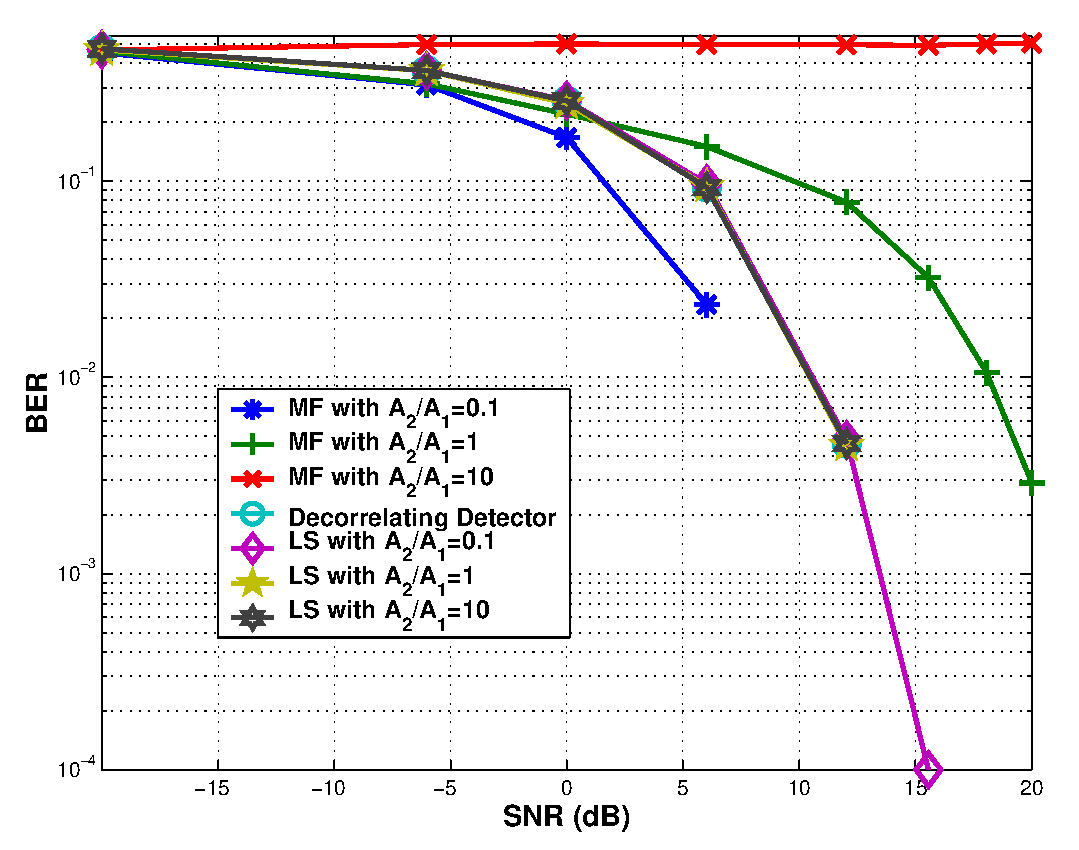
\includegraphics[width=3.25in]{SynchSemiBlindBER_LS0}}
\caption{BER comparison of the single-user matched filter,
decorrelating detector, and the LS semi-blind detector for the
first user in a two user system with $\rho=0.75$.} \label{BER_LS0}
\end{figure}

\subsection*{case 2: $\bar{\bN} \neq \mathbf{0}$}
%In this case, we are dealing some more practical situations. At
%this time,
It is assumed that the same level of AWGN exists in the semi-blind
signature matrix $\bcS$ as in the received signal $\br$.  The LS, TLS
and MLS semi-blind detectors are used to detect the information bit of
the desired user, $b_1$.
\begin{figure}
\center{
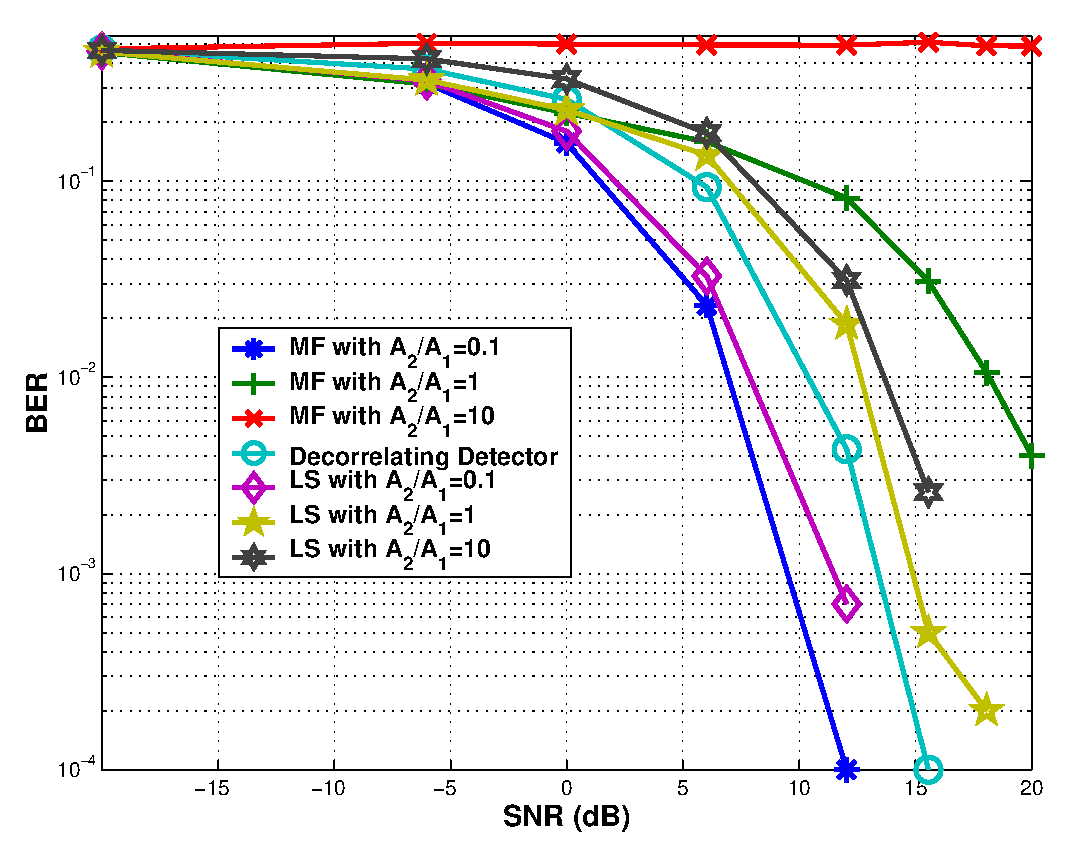
\includegraphics[width=3.25in]{SynchSemiBlindBER_LS1}}
\caption{BER comparison of the single-user matched filter,
decorrelating detector, and the LS semi-blind detector for the
first user in a two user system with $\rho=0.75$.} \label{BER_LS1}
\end{figure}
In Fig.~\ref{BER_LS1}, the performance of the LS semi-blind detector is
basically between that of decorrelating detector and single-user
matched-filter detector. The BER performance of all the detectors
becomes better when the SNR is increased. The difference from case 1 is
that when the MAI becomes strong, the performance of the LS detector
decreases.

\begin{figure}
\center{
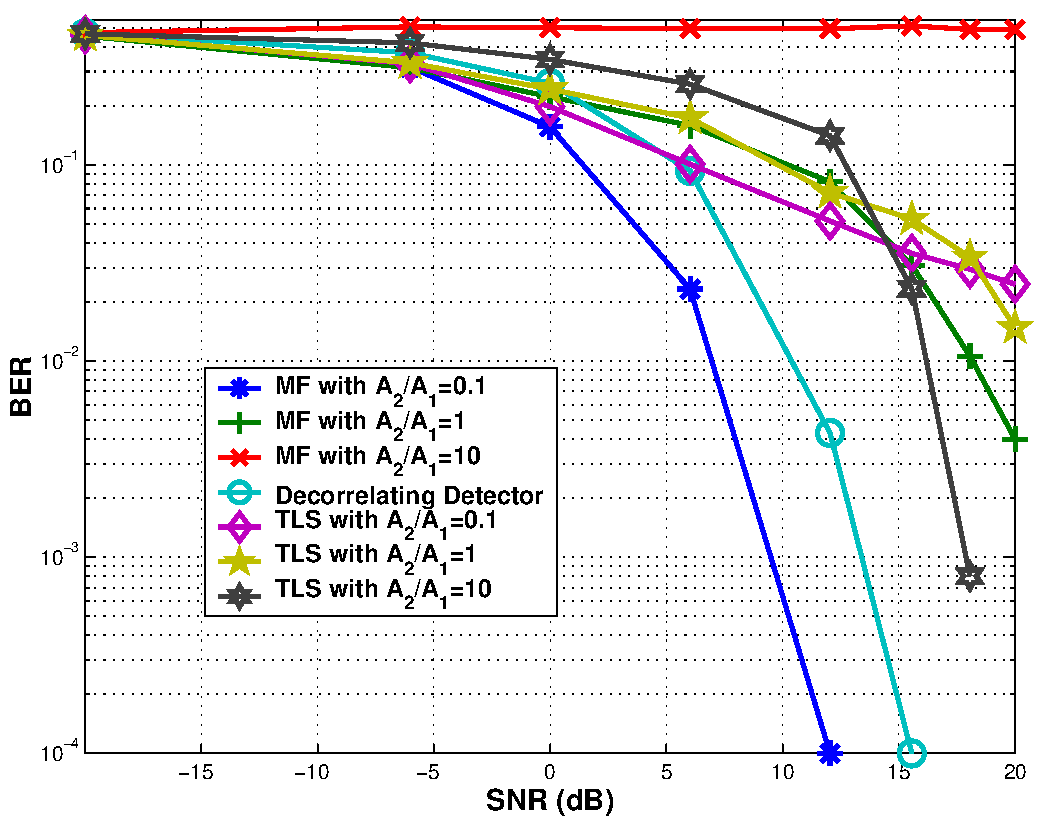
\includegraphics[width=3.25in]{SynchSemiBlindBER_TLS}}
\caption{BER comparison of the single-user matched filter,
decorrelating detector, and the TLS semi-blind detector for the
first user in a two user system with $\rho=0.75$.} \label{BER_TLS}
\end{figure}
In Fig.~\ref{BER_TLS}, the performance of the proposed TLS
semi-blind detector is evaluated. The BER performance of the TLS
detector becomes better when SNR is increased.  When the SNR is less
than $7$~dB, the BER performance of the TLS detector decreases with
increasing MAI.  But, when SNR is greater than about $12$~dB, the BER
performance of the TLS detector improves with increasing MAI. This
is different from the LS semi-blind detector.

\begin{figure}
\center{
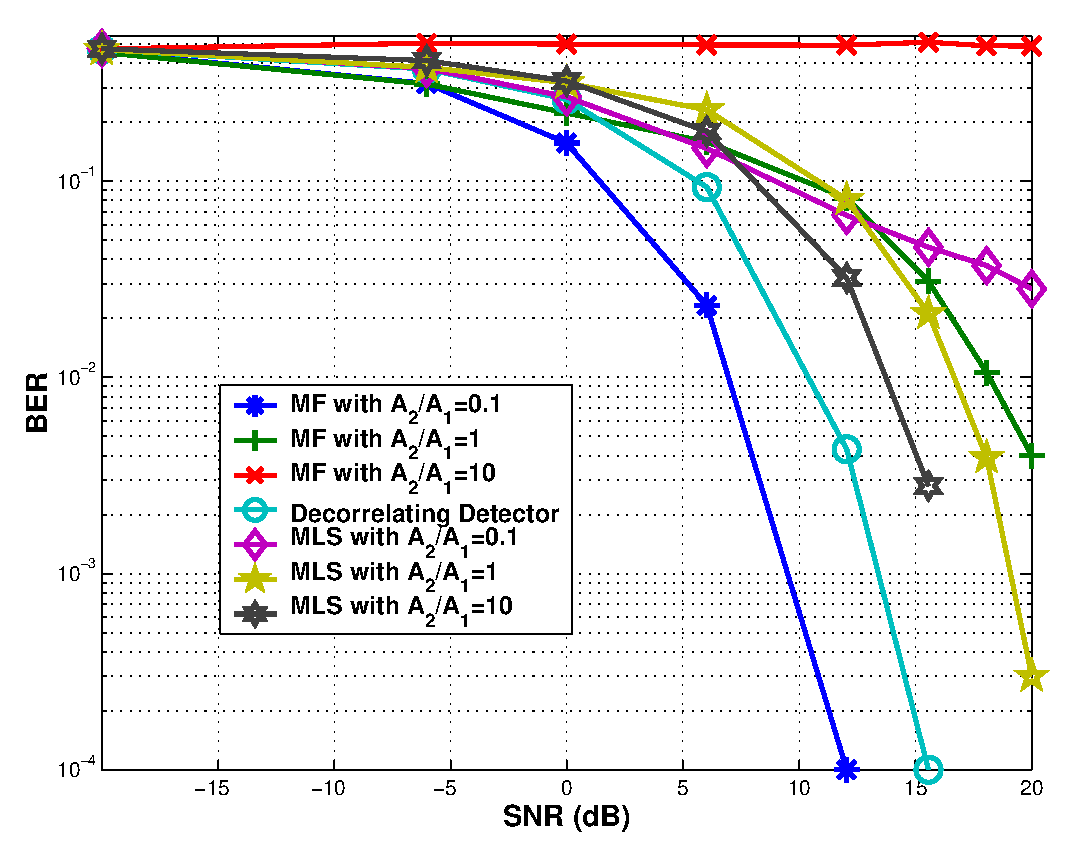
\includegraphics[width=3.25in]{SynchSemiBlindBER_MLS}}
\caption{BER comparison of the single-user matched filter,
decorrelating detector, and the MLS semi-blind detector for the
first user in a two user system with $\rho=0.75$.} \label{BER_MLS}
\end{figure}
The BER performance of the proposed MLS semi-blind detector is shown in
Fig.~\ref{BER_MLS}.  The BER performance of the MLS detector improves
with increasing SNR.  Similar to the TLS semi-blind detector, when the SNR
is less than $0$~dB, the BER performance of the MLS detector decreases
with increasing MAI.  When the SNR is greater than $13$~dB, the BER
performance of the MLS detector improves with increasing MAI.

\begin{figure}
\center{
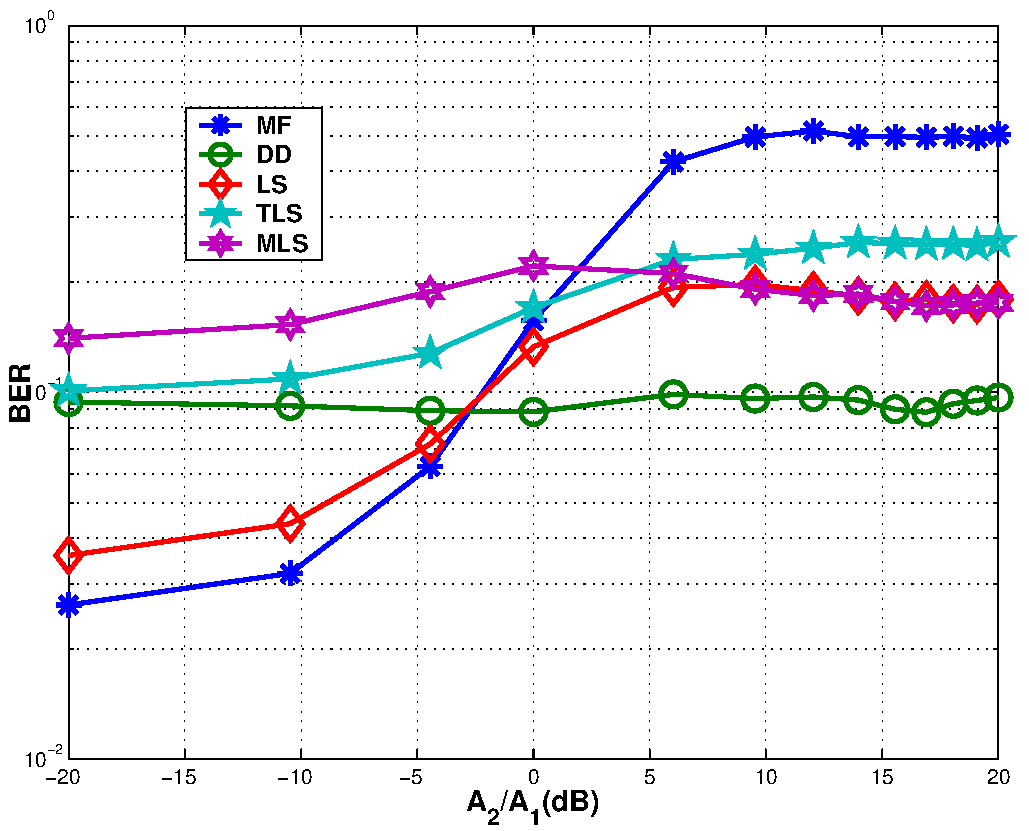
\includegraphics[width=3.25in]{SynchSemiBlindNFR}}
\caption{Near-far resistance comparison of the single-user matched
filter, decorrelating detector, and the LS, TLS and MLS semi-blind
detectors for the first user in a two user system with $\rho=0.75$
and $SNR=6dB$.} \label{NFR}
\end{figure}
In Fig.~\ref{NFR}, the BER curves of all the proposed detectors are shown
versus $A_2/A_1$ and are compared to the error probability of the
single-user matched filter detector and the decorrelating detector.
When $A_2/A_1<-5$~dB, both the LS and the MF detector work better than
the decorrelating detector.  But, the performance of the TLS and MLS
detectors are worse than that of the decorrelating detector in the same
region.  When $A_2/A_1>0$~dB, the performance of all the proposed
semi-blind detectors is close to that of the decorrelating detector and
much better than that of the single-user matched filter detector.
Further, the performance of the LS detector is better than that of the other
two proposed detectors.  We note that the MLS detector performs closely
to the LS detector.

\section{Conclusions}

In this paper, we presented the LS, TLS and MLS one-shot
semi-blind decorrelating detectors. In these semi-blind
decorrelating detectors, only the signature waveform and received amplitude
of the desired user are needed.  In the performance analysis and computer
simulations, the classic decorrelating detector is simply a special case of
the presented LS semi-blind decorrelating detector when there is
no noise in the semi-blind signature matrix.  Likewise, the single-user
matched filter is a special case when the SNR in the semi-blind signature
matrix is close to $0$.  The presented semi-blind decorrelating detectors
are one-shot algorithms which are simple and direct.  No searching or
adaptive procedure is required as in other semi-blind/blind detectors.

\bibliographystyle{unsrt}
\bibliography{WCNC03-SynchSemi}
\end{document}
